As discussed in Sec.~\ref{sec:pp_physics_jets}, color confinement prevents the existence of free quarks and gluons.
A quark or gluon produced at the LHC typically undergoes hadronization and presents itself in the detector as a collection of collimated particles.
Jets are built from PF candidates, using the anti-$k_{\text{T}}$ clustering algorithm~\cite{Cacciari:2008gp,Cacciari:2011ma} with a distance parameter of 0.4.
The input PF candidates have charged hadron subtraction (CHS) applied, meaning charged hadrons associated with vertices other than the primary vertex of that event are removed.
CHS reduces the contribution of particles originating from pileup vertices.
Once the jets are built from PF candidates, three steps are taken to correct the jets' energies.

First, a pileup offset correction is applied to remove additional jet contributions from pileup not removed by CHS.
The pileup contributions not remove by CHS are primarily charged hadrons not matched to a good vertex and PF photons.
The individual jet energies are corrected by a multiplicative factor derived in simulation, parametrized in bins of jet area ($A$), $\rho, \pT,$ and $\eta$.
Typical values for the pileup offset corrections are shown in Fig.~\ref{fig:evt_jet_pu_corrections}.
\begin{figure} [h!]
    \centering
    \begin{tabular}{c c}
        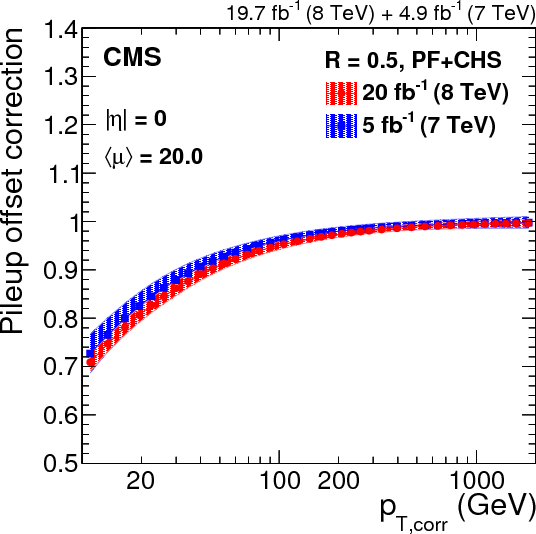
\includegraphics[width=0.48\linewidth]{figures/event_reconstruction_and_selection/jetmet8Tev_Figure_009-c.png} &
        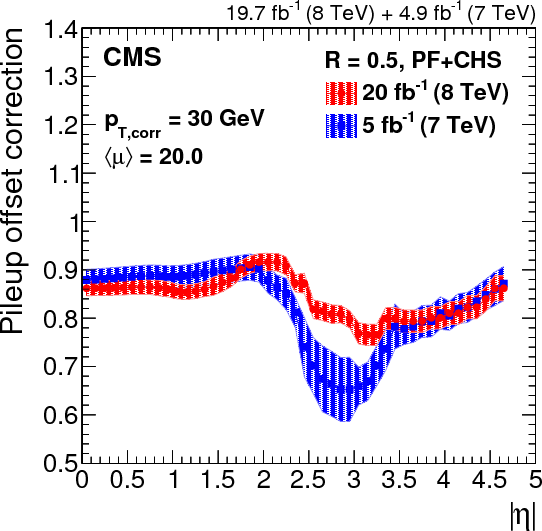
\includegraphics[width=0.48\linewidth]{figures/event_reconstruction_and_selection/jetmet8Tev_Figure_009-d.png}
    \end{tabular}
    \caption{Pileup offset correction values as a function of jet \pT (left) and jet $|\eta|$ (right). Taken from~\cite{Khachatryan_2017_jets}.}
    \label{fig:evt_jet_pu_corrections}
\end{figure}

Second, jet energy scale corrections designed to correct for the detector response to jets are derived in simulation, again in bins of jet area ($A$), $\rho, \pT,$ and $\eta$.
The goal of this step is to correct the reconstructed jet energy to match that of the true jet energy (only available in simulation).
Typical values for the jet energy scale corrections are shown in Fig.~\ref{fig:evt_jet_jec_corrections}. 
\begin{figure} [h!]
    \centering
    \begin{tabular}{c c}
        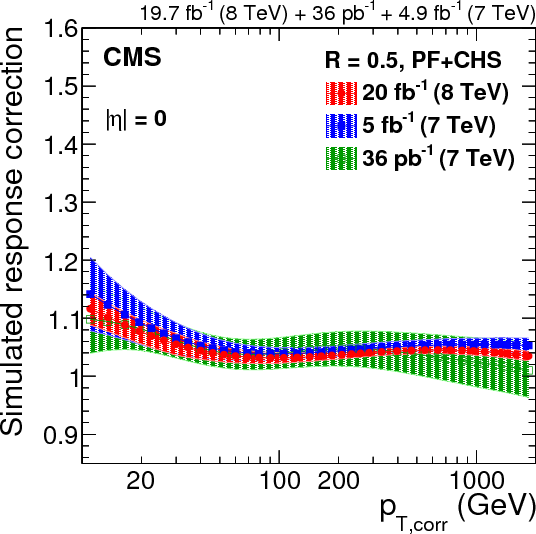
\includegraphics[width=0.48\linewidth]{figures/event_reconstruction_and_selection/jetmet8Tev_Figure_014-a.png} &
        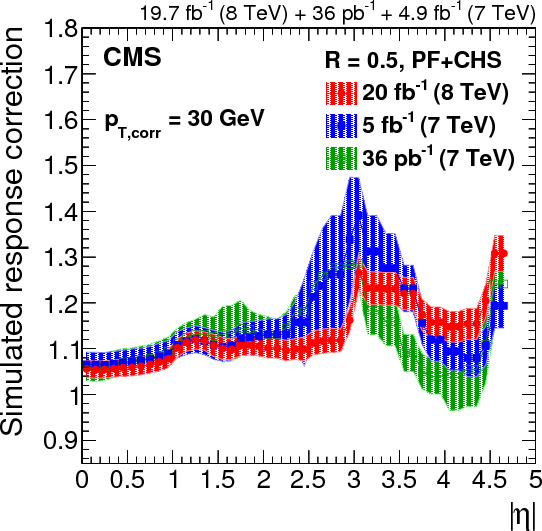
\includegraphics[width=0.48\linewidth]{figures/event_reconstruction_and_selection/jetmet8Tev_Figure_014-b.png}
    \end{tabular}
    \caption{Jet energy scale correction values as a function of jet \pT (left) and jet $|\eta|$ (right). Taken from~\cite{Khachatryan_2017_jets}.}
    \label{fig:evt_jet_jec_corrections}
\end{figure}

Third, remaining differences between data and simulation are corrected with a residual correction applied to data, derived as a function of \pT and $\eta$.
A variety of event topologies ($\gamma$ + jets, \Zee + jets, \Zuu + jets, and di-jet) are used to derive these corrections.
In each topology, the underlying strategy is the same: exploit the momentum conservation in the transverse plane betwen a well-measured reference object and the jet to be corrected.
The fact that the reference object ($\gamma$, \Zee, \Zuu, a well-measured central jet) is well-measured allows us to infer the true energy of the jet to be corrected.
The full details of these procedures are described in Ref.~\cite{Khachatryan_2017_jets}.

Jets used in the \ttH analysis are first corrected with the procedures described in this section.
They are further required to have $\pT > 25$ GeV and $|\eta| < 2.4$ and must pass a loose pileup jet ID criteria.
The loose pileup jet ID criteria is based on a BDT designed to discriminate between jets originating from pileup interactions and those originating from the primary vertex in the event.
The BDT is trained with variables describing the jets' shape as well as additional track information.
Jets are finally also required to not be overlapping with any photons or leptons in the event, requiring $\Delta R(\text{jet}, \text{photon/lepton}) > 0.4$.

\subsubsection*{b-Tagged Jets}
Hadronic jets at the LHC typically result from the hadronization of either a quark or gluon (with the exception of top quarks, which decay before they are able to hadronize).
Jets originating from a light-flavor quark (u,d,s) or a gluon are typically indistinguishable in the CMS detector.
However, jets originating from c or b quarks often have distinguishing features. 
While hadrons containing only light-flavor quarks (as would typically be produced by the hadronization of a light-flavor quark or a gluon) often reach the calorimeters before decaying, hadrons containing b quarks tend to decay on a length scale of a few millimeters when produced at typical LHC energies.
Hadrons containing charm quarks frequently decay even sooner than this.
The resolution of the tracker is sufficient to distinguish the vertices of these decays, called ``secondary vertices'', from the primary vertices in the event.

Jet flavor tagging algorithms attempt to exploit information about the secondary vertices associated with a given jet to determine the flavor of the quark (or gluon) it originated from.
Machine learning algorithms are often used to classify jet flavor, using information about the secondary vertices, tracks, and pf candidates associated with a given jet.
Recently, algorithms built with deep neural networks have shown significantly improved jet flavor tagging performance over more traditionally used methods, such as those based on boosted decision trees~\cite{Guest_2016}.
The DeepCSV~\cite{Sirunyan_2018_deepcsv} algorithm is one such DNN-based tagger.
For a given jet, the algorithm assigns multiple flavor scores, indicating its degree of certainty that the jet originated from a quark of that flavor.
DeepCSV outputs scores corresponding to its degree of certainty that the jet originated from a b quark, c quark, light flavor quark (u,d,s) or gluon, and a \bb pair (four scores).
The performance of DeepCSV (purple) and other commonly used jet flavor algorithms is shown in Fig.~\ref{fig:evt_jet_btag}.
\begin{figure} [h!]
    \centering
    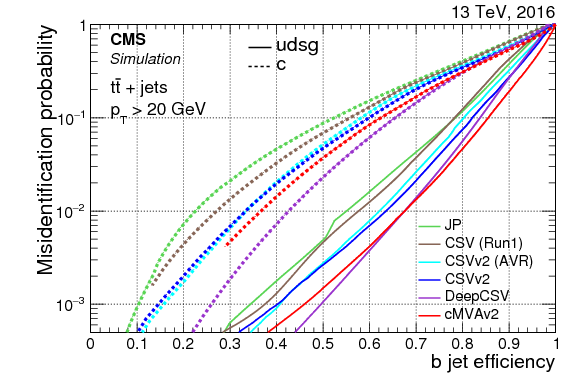
\includegraphics[width=\linewidth]{figures/event_reconstruction_and_selection/deepcsv_Figure_016.png}
    \caption{Misidentification rate as a function of b-tagging efficiency, shown for b vs. c jet discrimination (dotted lines) and b vs. light jet discrimination (solid lines). Taken from~\cite{Sirunyan_2018_deepcsv}.}
    \label{fig:evt_jet_btag}
\end{figure}

Jet flavor tagging is particularly useful for the \ttH analysis, as two b quarks are produced in the decay of the \ttb pair.
As the multi-jet, \gjets, and \dipho backgrounds primarily feature jets originating from light flavor quarks or gluons, the ability to select b-tagged jets allows for rejection of a significant component of the overall background.
